\documentclass[review]{elsarticle}
%-----------------------------------------------------

\usepackage{amsmath}
\usepackage{graphicx}

\graphicspath{{./figs/}}

\newcommand{\ihat}{\boldsymbol{\hat{\textbf{\i}}}}
\newcommand{\jhat}{\boldsymbol{\hat{\textbf{\j}}}}
\newcommand{\roughly}{{\raise.17ex\hbox{$\scriptstyle\sim$}}}
\newcommand{\dmax}{d_\text{max}}
\newcommand{\dmin}{d_\text{min}}

%-----------------------------------------------------

\makeatletter
\renewcommand{\fnum@figure}{Figure 5}
\makeatother

\thispagestyle{empty}

\begin{document}
\allowdisplaybreaks

\begin{figure}[ht]
\centering
%\includegraphics[width=\textwidth]{Figure_05_HR.pdf}
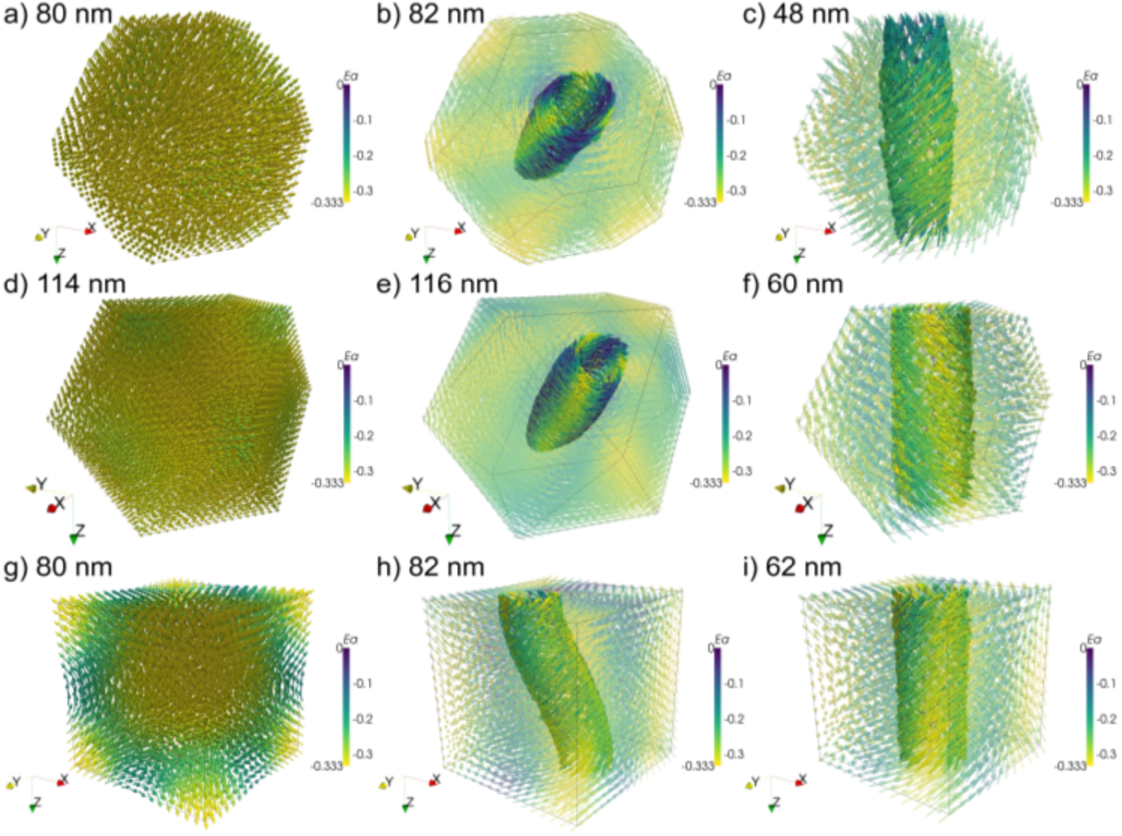
\includegraphics[width=\textwidth]{Figure_05.pdf}
\caption{Micromagnetic structures of maximally truncated octahedra, cuboctahedra and cubes. Left column (a, d, g) shows the largest SD solutions at $\dmax$, obtained by interpolating from solutions for smaller grains starting at 30$\,\text{nm}$. On interpolating to a grain 2$\,\text{nm}$ larger, the structures relax to an EAV (b, e) or a distorted EAV (h) which are stable up to 120$\,\text{nm}$. From 120$\,\text{nm}$ interpolation is carried out into smaller grains. Eventually the vortex aligns with a hard direction (c, f, i), stable down to $\dmin$ after which the solution becomes SD again down to 30$\,\text{nm}$. Top row (a, b, c) shows the structures for the maximally truncated octahedra; center row (d, e, f) for the cuboctahedra and bottom row (g, h, i) for the cubes. Colour represents the MCA energy normalised by $|K_1|$.}
\label{fig5}
\end{figure}

\end{document}